\section{多孔催化剂中的扩散与反应}


\begin{frame}
    \frametitle{多孔催化剂中的扩散与反应}

        \begin{minipage}{0.48\linewidth}
            在多相催化反应中，反应物分子从气相主体穿过颗粒外表面的层流边界层，到达催化剂外表面后，一部分反应物即开始反应。由于固体催化剂的多孔性，由颗粒内部孔道壁面所构成的内表面要比颗粒外表面大得多。
        \end{minipage}\hfill
        \begin{minipage}{0.48\linewidth}
            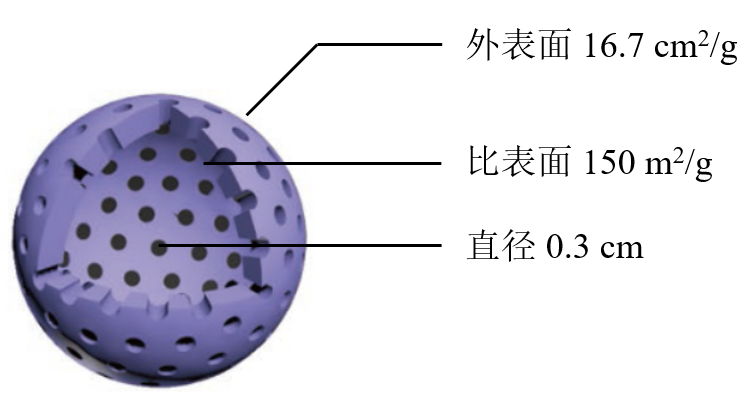
\includegraphics[width=\linewidth]{figures/surface.png}
        \end{minipage}

        所以，绝大多数反应物分子要沿着孔道向颗粒内部扩散，即所谓\highlight{内扩散}。与外扩散不同的是，外扩散时反应物要先扩散到颗粒外表面才可发生反应，而内扩散是与反应并行进行的，即反应物沿着孔道空间向粒内深处扩散的同时，就有反应物分子在孔壁面上发生催化反应。随着扩散的进行，由于克服扩散阻力以及反应消耗，反应物的浓度逐渐下降，反应速率也相应地降低，到颗粒中心时反应物浓度最低（或等于零），反应速率也最小。

\end{frame}


\begin{frame}
    \frametitle{多孔催化剂中的扩散与反应}

    如果反应速率较慢，而反应组分的有效扩散系数又较大，则孔道内外只需很小的浓度差，便能供给孔内表面反应所消耗的反应物，孔壁各处所接触的反应物浓度几乎都等于孔口处的浓度，通常认为这时整个颗粒的内表面都得到了充分的利用。
    
    反之，若反应速率相当快，反应物进入孔道内不长的距离即已反应完全（不可逆反应），为了供给孔内表面反应消耗的反应物，孔内外需有相当大的浓度梯度，且反应大部分是在颗粒表层的一定厚度的壳层中进行，其余部分由于反应物浓度甚小，它对反应的贡献就甚微，这时颗粒内表面没有得到充分的利用。

    \bigskip
    
    多孔催化剂内反应组分的浓度分布是不均匀的，温度一定时，浓度的高低直接影响反应速率的大小。所以，确定催化剂颗粒内反应组分的浓度分布就十分必要。

\end{frame}


\begin{frame}
    \frametitle{多孔催化剂内反应组分的浓度分布}

        \begin{minipage}{0.65\linewidth}
            考察如图所示的薄片催化剂，在其上进行一级不可逆反应。设该催化剂颗粒是等温的，且其孔隙结构均匀，各向同性。为了确定颗粒内反应物A的浓度分布，需先建立描述此过程的反应---扩散微分方程。为此，可在颗粒内取一厚度为$\dif Z$的微元，对此微元作反应物A的物料衡算即可。

            \bigskip
            
            \quad 单位时间内扩散进入微元的组分A量

            $-$单位时间内由微元扩散出的组分A量

            $=$在微元内反应掉的组分A量
        \end{minipage}\hfill
        \begin{minipage}{0.32\linewidth}
            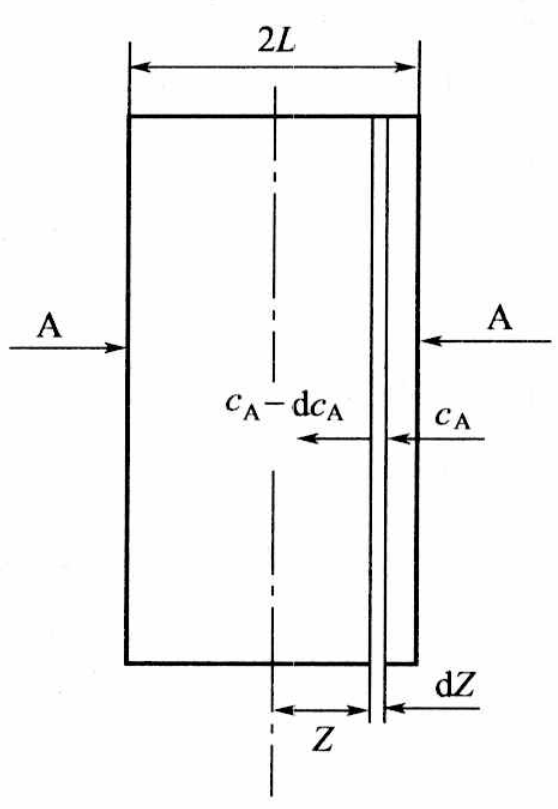
\includegraphics[width=\linewidth]{figures/fig6.3.png}
        \end{minipage}

\end{frame}


\begin{frame}
    \frametitle{多孔催化剂内反应组分的浓度分布}

        \begin{minipage}{0.65\linewidth}
            设有效扩散系数$D_\mathrm{e}$为常数，扩散面积为$a$，则
            \[
                D_{\mathrm{e}} a\left(\frac{\mathrm{d} c_{\mathrm{A}}}{\mathrm{d} Z}\right)_{\mathrm{Z}+\mathrm{d} Z}-D_{\mathrm{e}} a\left(\frac{\mathrm{d} c_{\mathrm{A}}}{\mathrm{d} Z}\right)_{\mathrm{Z}}=k_{\mathrm{p}} c_{\mathrm{A}} a \mathrm{~d} Z
            \]
            $k_\mathrm{p}$系以催化剂颗粒体积为基准的反应速率常数。
            \[
                \left(\frac{\mathrm{d} c_{\mathrm{A}}}{\mathrm{d} Z}\right)_{\mathrm{Z}+\mathrm{d} Z}=\left(\frac{\mathrm{d} c_{\mathrm{A}}}{\mathrm{d} Z}\right)_{\mathrm{Z}}+\frac{\mathrm{d}}{\mathrm{d} Z}\left(\frac{\mathrm{d} c_{\mathrm{A}}}{\mathrm{d} Z}\right) \mathrm{d} Z
            \]
            代入化简后得
            \[
                \frac{\mathrm{d}^{2} c_{\mathrm{A}}}{\mathrm{d} Z^{2}}=\frac{k_{\mathrm{p}}}{D_{\mathrm{e}}} c_{\mathrm{A}}
            \]
            这就是薄片催化剂上进行一级不可逆反应时的反应扩散方程。
        \end{minipage}\hfill
        \begin{minipage}{0.32\linewidth}
            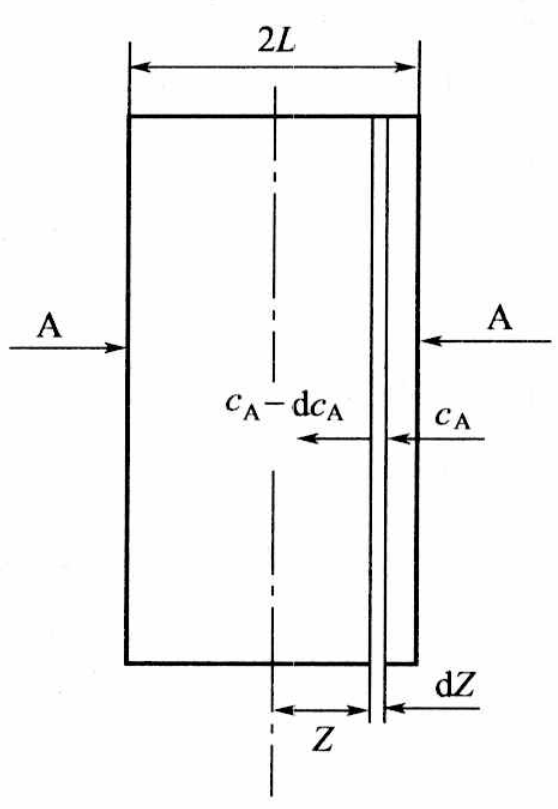
\includegraphics[width=\linewidth]{figures/fig6.3.png}
        \end{minipage}

\end{frame}


\begin{frame}
    \frametitle{多孔催化剂内反应组分的浓度分布}

    结合其边界条件 $\begin{cases}    
        Z=L, c_{\mathrm{A}}=c_{\mathrm{AS}} \\
    
        Z=0, \mathrm{~d} c_{\mathrm{A}} / \mathrm{d} Z=0    
    \end{cases}$

    解之得催化剂颗粒内反应物的浓度分布。

    引入下列无量纲量
    \[
        \xi=c_{\mathrm{A}} / c_{\mathrm{AS}}, \quad \zeta=Z / L, \quad \phi^{2}=L^{2} \frac{k_{p}}{D_{\mathrm{e}}}
    \]
    无量纲化得
    \[
        \frac{\mathrm{d}^{2} \xi}{\mathrm{d} \zeta^{2}}=\phi^{2} \xi
    \]
    \[
        \zeta=1 \qquad \qquad \xi=1
    \]
    \[
        \zeta=0 \quad \mathrm{~d} \xi / \mathrm{d} \zeta=0
    \]

\end{frame}


\begin{frame}
    \frametitle{多孔催化剂内反应组分的浓度分布}

    上式为二阶常系数线性齐次微分方程，其通解为
    \[
        \xi=A \mathrm{e}^{\phi \zeta}+B \mathrm{e}^{-\phi \zeta}
    \]
    结合边界条件，可求得积分常数A及B为
    \[
        \mathrm{A}=\mathrm{B}=1 /(\mathrm{e}^{\phi}+\mathrm{e}^{-\phi})
    \]
    代回，得
    \[
        \xi=\frac{\mathrm{e}^{\phi \zeta}+\mathrm{e}^{-\phi \zeta}}{\mathrm{e}^{\phi}+\mathrm{e}^{-\phi}}=\frac{\cosh (\phi \zeta)}{\cosh (\phi)}
    \]
    或
    \[
        \frac{c_{\mathrm{A}}}{c_{\mathrm{AS}}}=\frac{\cosh (\phi Z / L)}{\cosh (\phi)}
    \]
    这便是薄片催化剂内反应物的浓度分布方程。

\end{frame}


\begin{frame}
    \frametitle{多孔催化剂内反应组分的浓度分布}

        \begin{minipage}{0.55\linewidth}
            为了直观地考察其变化规律，以$\phi $为参数，以$\xi$对$\zeta$作图，如图所示。
            \begin{itemize}
                \item 无论$\phi $为何值，无量纲浓度$\xi$总是随无量纲距离$\zeta$的减小而降低，即从颗粒外表面到颗粒中心处反应物A的浓度逐渐降低。
                \item $\phi $值不同，其降低的程度也不同：$\phi $值越大，反应物的浓度变化越急剧。
            \end{itemize}
        \end{minipage}\hfill
        \begin{minipage}{0.4\linewidth}
            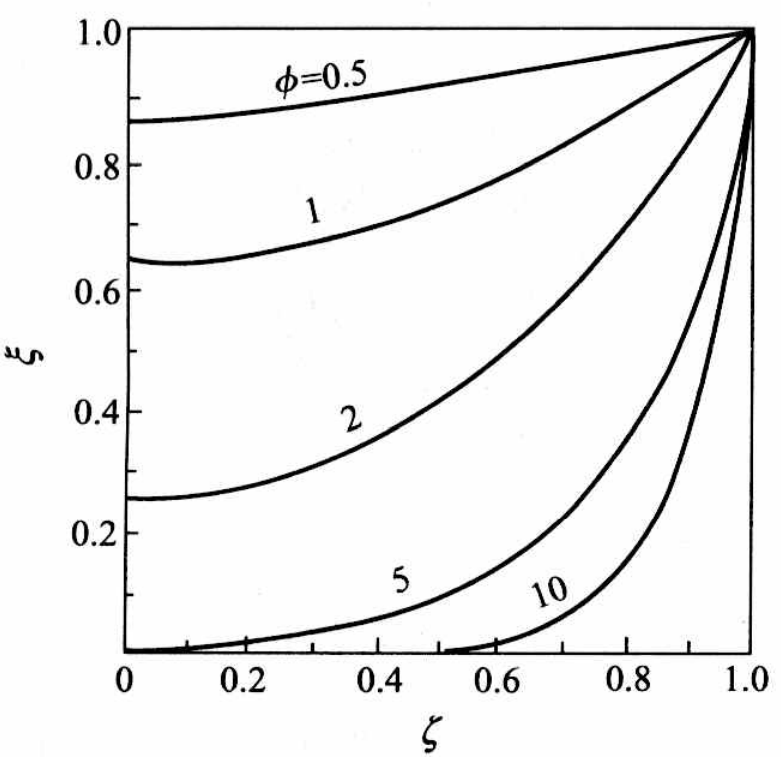
\includegraphics[width=\linewidth]{figures/fig6.4.png}
        \end{minipage}

        颗粒内的浓度分布是反应物的扩散与反应综合作用的结果，而$\phi $值的大小又反映了浓度分布的特征，从$\phi $值可以判断内扩散对反应过程的影响程度。

\end{frame}


\begin{frame}
    \frametitle{多孔催化剂内反应组分的浓度分布}

    无量纲参数$\phi$叫做梯尔(Thiele)模数，是处理扩散与反应问题的一个极其重要的特征参数。
    
    根据前面对梯尔模数所下的定义，作适当的改写可得其物理意义为
    \[
        \phi^{2}=L^{2} \frac{k_{\mathrm{p}}}{D_{\mathrm{e}}}=\frac{a L k_{\mathrm{p}} c_{\mathrm{AS}}}{D_{\mathrm{e}} a(c_{\mathrm{AS}}-0) / L}=\frac{\text { 表面反应速率 }}{\text { 内扩散速率 }} 
    \]
    由此可知梯尔模数表示表面反应速率与内扩散速率的相对大小。
    \begin{itemize}
        \item $\phi$值越大，表明表面反应速率大而内扩散速率小，
        
        说明内扩散阻力对反应过程的影响大。
        \item $\phi$值越小，说明内扩散阻力对反应过程的影响越小。
    \end{itemize}
    
\end{frame}


\begin{frame}
    \frametitle{内扩散有效因子}

    为了计算催化剂颗粒上的反应速率，引用内扩散有效因子$\eta$，其定义如下
    \[
        \eta=\frac{\text { 内扩散对过程有影响时的反应速率 }}{\text { 内扩散对过程无影响时的反应速率 }} 
    \]
    内扩散有影响时催化剂颗粒内的浓度是不均匀的，需求出此时的平均反应速率
    \[
        \left\langle r_{\mathrm{A}}\right\rangle=\frac{1}{L} \int_{0}^{L} k_{\mathrm{p}} c_{\mathrm{A}} \mathrm{d} Z
    \]
    将$\frac{c_{\mathrm{A}}}{c_{\mathrm{A}_{\mathrm{S}}}}=\frac{\cosh (\phi Z / L)}{\cosh (\phi)}$代入，得
    \[
        \left\langle r_{\mathrm{A}}\right\rangle=\frac{k_{\mathrm{p}} c_{\mathrm{AS}}}{L \cos h \phi} \int_{0}^{L} \cosh (\phi Z / L) \mathrm{d} Z=\frac{k_{\mathrm{p}} c_{\mathrm{AS}} \tan h(\phi)}{\phi}
    \]
    这即为内扩散有影响时的反应速率。

\end{frame}


\begin{frame}
    \frametitle{内扩散有效因子}

    内扩散没有影响时，颗粒内部处的浓度均与外表面上的浓度$c_{\mathrm{AS}}$相等，因之，相应的反应速率为$k_{\mathrm{p}}c_{\mathrm{AS}}$，把这两个反应速率代入内扩散有效因子定义式，化简后可得
    \[
        \eta=\tanh (\phi) / \phi 
    \]
    这便是在薄片催化剂上进行一级不可逆反应时，内扩散有效因子的计算公式。
    \begin{minipage}{0.48\linewidth}
        \begin{itemize}
            \item $\eta$值总是随$\phi$值的增大而单调地下降
            \item $\phi$值越大，内扩散的影响也越大
            \item 减小催化剂颗粒的尺寸，$\phi$值减小
            \item 增大催化剂的孔容和孔半径，可提高有效扩散系数$D_\mathrm{e}$的值，从而使$\phi$值减小
        \end{itemize}
    \end{minipage}\hfill
    \begin{minipage}{0.48\linewidth}
        \begin{figure}[htpb]
            \centering
            
\includegraphics[width=.8\linewidth]{薄片}
        \end{figure}
    \end{minipage}
\end{frame}


\begin{frame}
    \frametitle{内扩散有效因子}

    综上所述，内扩散有效因子计算式的推导可概括为如下几步：
    \begin{enumerate}
        \item 建立催化剂颗粒内反应物浓度分布的微分方程，即扩散反应方程，确定相应的边界条件；解此微分方程而求得浓度分布；
        \item 根据浓度分布而求得颗粒内的平均反应速率；
        \item 由内扩散有效因子的定义即可导出其计算式。
    \end{enumerate}

    按此步骤可导出其他几何形状的催化剂颗粒的内扩散有效因子计算式。

\end{frame}


\begin{frame}
    \frametitle{内扩散有效因子}

    对于半径为$R_\mathrm{p}$的球形催化剂粒子，在粒内进行等温一级不可逆反应，取任一半径$r$处厚度为$\dif r$的壳层，对组分A作物料衡算。其扩散反应方程为
        \begin{minipage}{0.55\linewidth}
            \[
                \frac{\mathrm{d}^{2} c_{\mathrm{A}}}{\mathrm{d} r^{2}}+\frac{2}{r} \frac{\mathrm{d} c_{\mathrm{A}}}{\mathrm{d} r}=\frac{k_{\mathrm{p}}}{D_{\mathrm{e}}} c_{\mathrm{A}}
            \]
            对于半径为$R_\mathrm{p}$的无限长圆柱或两端面无孔的有限长圆柱，其扩散反应方程为
            \[
                \frac{\mathrm{d}^{2} c_{\mathrm{A}}}{\mathrm{d} r^{2}}+\frac{1}{r} \frac{\mathrm{d} c_{\mathrm{A}}}{\mathrm{d} r}=\frac{k_{\mathrm{p}}}{D_{\mathrm{e}}} c_{\mathrm{A}}
            \]            
        \end{minipage}\hfill
        \begin{minipage}{0.42\linewidth}
            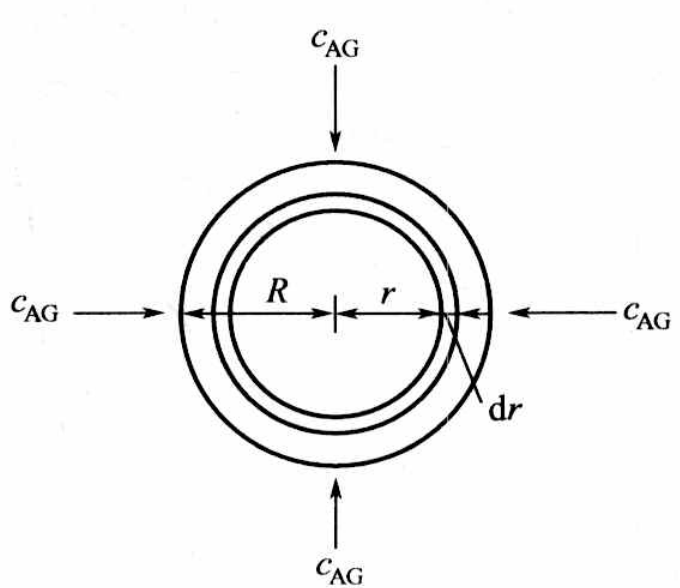
\includegraphics[width=\linewidth]{figures/fig6.6.png}
        \end{minipage}

\end{frame}


\begin{frame}
    \frametitle{内扩散有效因子}

    无论球形还是圆柱，都可采用下列边界条件
    \[
        r=R_{\mathrm{p}}, \quad c_{\mathrm{A}}=c_{\mathrm{AS}}
    \]
    \[
        r=0, \quad \mathrm{~d} c_{\mathrm{A}} / \mathrm{d} r=0
    \]
    结合给定的边界条件，这两个方程的解分别为
    \[
        \text{圆球：} \qquad \frac{c_{\mathrm{A}}}{c_{\mathrm{AS}}}=\frac{R_{\mathrm{p}} \sin h\left(3 \phi r / R_{\mathrm{p}}\right)}{r \sin h(3 \phi)}
    \]
    \[
        \text{圆柱：} \qquad \frac{c_{\mathrm{A}}}{c_{\mathrm{AS}}}=\frac{I_{0}\left(2 \phi r / R_{\mathrm{p}}\right)}{I_{0}(2 \phi)} \qquad ~
    \]
    式中$I_{0}$为零阶一类变型贝塞尔函数。

\end{frame}


\begin{frame}
    \frametitle{内扩散有效因子}

    式中$\phi$为适用于不同几何形状的催化剂颗粒的梯尔模数
    \[
        \phi=\frac{V_{\mathrm{p}}}{a_{\mathrm{p}}} \sqrt{\frac{k_{\mathrm{p}}}{D_{\mathrm{e}}}}
    \]
    其中$V_{\mathrm{p}}$和$a_{\mathrm{p}}$分别为颗粒的体积与外表面积，此式与前面对薄片催化剂而定义的梯尔模数完全一致。

    根据浓度分布式分别求出粒内平均反应速率，再用定义式即可导出圆球及圆柱的内扩散有效因子计算式如下：
    \[
        \text{圆球：} \qquad \eta =\frac{1}{\phi}\left[\frac{1}{\tan h(3 \phi)}-\frac{1}{3 \phi}\right]
    \]
    \[
        \text{圆柱：} \qquad \eta =I_{1}(2 \phi) /\left[\phi I_{0}(2 \phi)\right] \quad
    \]
    式中$I_{1}$为一阶一类变型贝塞尔函数，其值可从贝塞尔函数表中查得。

\end{frame}


\begin{frame}
    \frametitle{内扩散有效因子}
        \begin{minipage}{0.55\linewidth}
            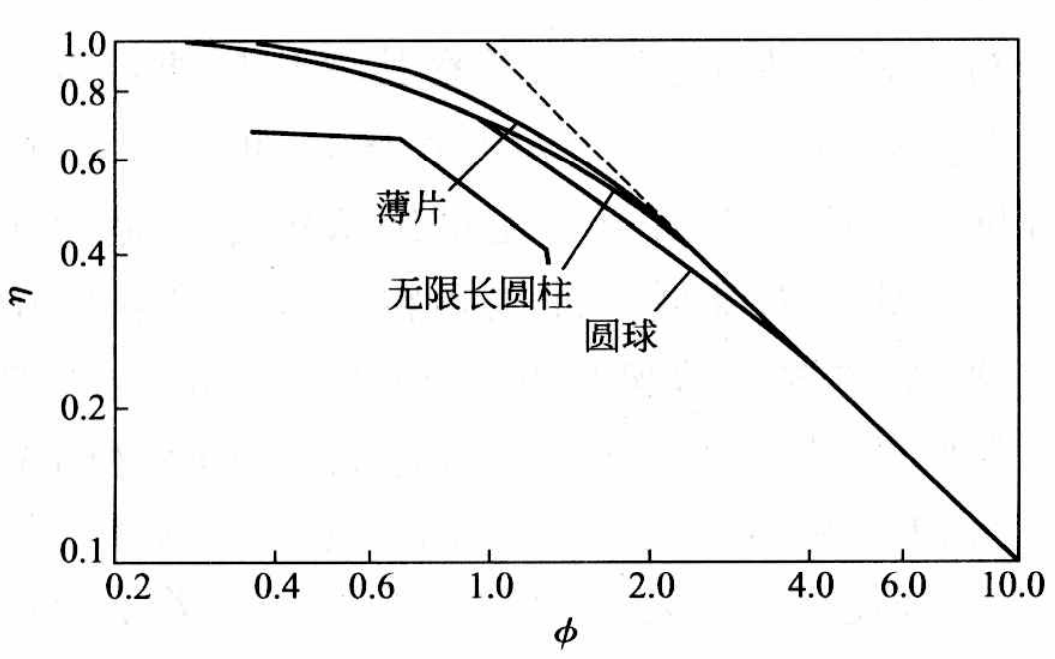
\includegraphics[width=\linewidth]{figures/fig6.5.png}
        \end{minipage}\hfill
        \begin{minipage}{0.4\linewidth}
            比较不同几何形状的催化剂颗粒的内扩散有效因子，图上三条曲线几乎重合为一，特别是值较小或值较大时更为明显。
        \end{minipage}
        
        只有当$0.4 < \phi <3$时，三者才有较明显的差别。纵使在这一区域内，它们之间相差只不过$10\% \sim 20\%$。
    
    所以，对任何几何形状的催化剂颗粒，均可按前述$\eta$计算式计算得到可接受的内扩散有效因子值。
            
\end{frame}


\begin{frame}
    \frametitle{内扩散有效因子}

    无论是何种形状的催化剂颗粒，
    \begin{itemize}
        \item 当$\phi<0.4$时，$\eta \approx 1$，即内扩散的影响可忽略。
        \item 当$\phi>3.0$时，即内扩散影响严重时，三条曲线与其渐近线（图中的虚线）
        相重合，此时$$\eta = 1/\phi$$

        在此情况下，对于任何形状的催化剂颗粒，都可用此式来估算内扩散有效因子。
    \end{itemize}

    最后需要再次指出，\bf{以上的讨论只适用于等温下进行一级不可逆反应的情况}。

\end{frame}


\begin{frame}[t]
    \frametitle{}
    \begin{example}
        乙烯直接水合制乙醇的初始反应速率符合一级反应动力学方程。在300℃，7.0 MPa时，其反应速率常数为0.09 s$^{-1}$。催化剂颗粒直径为5 mm，有效扩散系数$D_\mathrm{e} = 7.04\times 10^{-4}$ \si{cm^2/s}。试求催化剂颗粒的内部效率因子。
    \end{example}
\end{frame}


\begin{frame}[t]
    \frametitle{}

    \begin{example}
        在铬铝催化剂上进行丁烷脱氢反应，其反应速率方程为
        \[
            r_{\mathrm{A}} =k_{\mathrm{W}} c_{\mathrm{A}} \quad \mathrm{mol} /(\mathrm{g} \cdot \mathrm{s})
        \]
        0.1013 MPa及773 K时，$k_\mathrm{W} = \SI{0.92}{cm^3/(g.s)}$。若在该温度下采用厚度为8 mm的薄片催化剂进行反应，催化剂平均孔半径为\SI{48e-10}{m}，孔容为\SI{0.35}{cm^3/g}，曲节因子等于2.5。试计算内扩散有效因子。
    \end{example}
    \only<2>{
    $\begin{aligned}
        \frac{\lambda}{2 r_{\mathrm{a}}} &=\frac{10^{-5}}{2 \times 48 \times 10^{-8}}=10.4>10 \\
        D_{\mathrm{K}} &=9700\left(48 \times 10^{-8}\right)(773 / 58)^{1 / 2}=1.70 \times 10^{-2} \mathrm{~cm}^{2} / \mathrm{s} \\
        D_{\mathrm{eA}} &=V_{\mathrm{g}} \rho_{\mathrm{p}} D_{\mathrm{K}} / \tau_{\mathrm{m}}=0.35\left(1.70 \times 10^{-2}\right) \rho_{\mathrm{p}} / 2.5=2.38 \times 10^{-3} \rho_{\mathrm{p}} \quad \mathrm{cm}^{2} / \mathrm{s} \\
        k_{\mathrm{p}} &=k_{\mathrm{W}} \rho_{\mathrm{p}}=0.92 \rho_{\mathrm{p}} \quad \mathrm{s}^{-1}
        \end{aligned}$
        }
        \only<3>{
            $\begin{aligned}        
                \phi &=\frac{0.8}{2}(\frac{0.92 \rho_{\mathrm{p}}}{2.38 \times 10^{-3} \rho_{\mathrm{p}}})^{1 / 2}=7.86 \\
                \eta &= \tanh (7.86)/7.86 = 0.127
            \end{aligned}$
        
            由于$\phi = 7.86>3$，内扩散影响相当严重，用简化式计算$\eta$所得的值与用精确式计算完全一致。
            }
\end{frame}



\begin{frame}[t]
    \frametitle{}

    \begin{example}
       在等温球形催化剂上进行一级可逆反应\ch{A <=> B}，试推导内扩散有效因子计算式。
    \end{example}

\end{frame}


\begin{frame}
    \frametitle{非一级反应的内扩散有效因子}

    处理非一级反应的扩散反应问题，原则上，前面所采用的方法与步骤完全适用，只是在数学处理上比较繁琐。

    设在等温薄片催化剂上进行某一化学反应，其速率方程为
    \[
        r_{\mathrm{A}}=k_{\mathrm{p}} f(c_{\mathrm{A}})
    \]
    设有效扩散系数$D_\mathrm{e}$为常数，扩散反应方程为
    \[
        \frac{\mathrm{d}^{2} c_{\mathrm{A}}}{\mathrm{d} Z^{2}}=\frac{k_{\mathrm{p}}}{D_{\mathrm{e}}} f(c_{\mathrm{A}})
    \]
    \[
        \text{因} \quad \frac{\mathrm{d}^{2} c_{\mathrm{A}}}{\mathrm{d} Z^{2}}=\frac{\mathrm{d} c_{\mathrm{A}}}{\mathrm{d} Z}\left[\frac{\mathrm{d}}{\mathrm{d} c_{\mathrm{A}}} \times \frac{\mathrm{d} c_{\mathrm{A}}}{\mathrm{d} Z}\right] \quad \text{并设} \quad p = \dif c_\mathrm{A}/\dif Z \quad \text{则}
    \]
    \[
        p \frac{\mathrm{d} p}{\mathrm{~d} c_{\mathrm{A}}}=\frac{k_{\mathrm{p}}}{D_{\mathrm{e}}} f(c_{\mathrm{A}})
    \]

\end{frame}


\begin{frame}
    \frametitle{非一级反应的内扩散有效因子}

    \[
        z=L \quad c_{\mathrm{A}}=c_{\mathrm{AS}} \quad p=p_{\mathrm{S}}=(\mathrm{d} c_{\mathrm{A}} / \mathrm{d} Z)_{\mathrm{S}}
    \]
    \[
        z=0 \quad c_{\mathrm{A}}=c_{\mathrm{AC}}=\dif c_{\mathrm{A}} / \mathrm{d} Z=0 \qquad \quad
    \]
    积分$p \frac{\mathrm{d} p}{\mathrm{~d} c_{\mathrm{A}}}=\frac{k_{\mathrm{p}}}{D_{\mathrm{e}}} f(c_{\mathrm{A}})$得
    \[
        p_{\mathrm{S}}=\left(\frac{\mathrm{d} c_{\mathrm{A}}}{\mathrm{d} Z}\right)_{\mathrm{S}}=\left[\frac{2 k_{\mathrm{p}}}{D_{\mathrm{e}}} \int_{c_{\mathrm{AC}}}^{c_{\mathrm{AS}}} f(c_{\mathrm{A}}) \mathrm{d} c_{\mathrm{A}}\right]^{1 / 2}
    \]
    扩散进入催化剂颗粒的组分A量为
    \[
        D_{\mathrm{e}} a_{\mathrm{p}}\left(\frac{\mathrm{d} c_{\mathrm{A}}}{\mathrm{d} Z}\right)_{\mathrm{S}}=D_{\mathrm{e}} a_{\mathrm{p}}\left[\frac{2 k_{\mathrm{p}}}{D_{\mathrm{e}}} \int_{c_{\mathrm{AC}}}^{c_{\mathrm{AS}}} f(c_{\mathrm{A}}) \mathrm{d} c_{\mathrm{A}}\right]^{1 / 2}
    \]
    对于定态过程，这也等于在颗粒内起反应的组分A量。

\end{frame}


\begin{frame}
    \frametitle{非一级反应的内扩散有效因子}

    如果内扩散没有影响，则催化剂颗粒内组分A的浓度与外表面处的浓度$c_{\mathrm{AS}}$相等，相应起反应的组分A量应为$La_\mathrm{p}k_\mathrm{p}f(c_{\mathrm{AS}})$。将这两个量代入定义式整理后可得内扩散有效因子为
    \[
        \eta=\frac{\sqrt{2 D_{\mathrm{e}}}}{L \sqrt{k_{\mathrm{p}}} f(c_{\mathrm{AS}})}\left[\int_{c_{\mathrm{AC}}}^{c_{\mathrm{AS}}} f(c_{\mathrm{A}}) \mathrm{d} c_{\mathrm{A}}\right]^{1 / 2}
    \]
    用此式来计算最大的困难是催化剂中心浓度未知，也难以用实验测定。
    
    当内扩散影响大时，对于不可逆反应，颗粒中心浓度$c_{\mathrm{AC}} \approx 0$；
    
    对于可逆反应，则$c_{\mathrm{AC}} \approx  c_{\mathrm{Ae}}$，而$c_{\mathrm{Ae}}$是可以计算出来的。
    \[
        \eta=\frac{a_{\mathrm{p}} \sqrt{2 D_{\mathrm{e}}}}{V_{\mathrm{p}} \sqrt{k_{\mathrm{p}}} f(c_{\mathrm{AS}})}\left[\int_{c_{\mathrm{AC}}}^{c_{\mathrm{AS}}} f(c_{\mathrm{A}}) \mathrm{d} c_{\mathrm{A}}\right]^{1 / 2}
    \]
    此式可用于其他几何形状的催化剂颗粒。

\end{frame}


\begin{frame}
    \frametitle{内外扩散都有影响时的有效因子}

    若反应过程中内、外扩散都有影响，则定义总有效因子为
    \[
        \eta_0 = \frac{\text{内外扩散都有影响时的反应速率}}{\text{无扩散影响时的反应速率}}
    \]
    对一级反应可以写出
    \[
        (-\mathscr{R}_{\mathrm{A}})=k_{\mathrm{G}} a_{\mathrm{m}}(c_{\mathrm{AG}}-c_{\mathrm{AS}})=\eta k_{\mathrm{W}} c_{\mathrm{AS}}=\eta_{0} k_{\mathrm{W}} c_{\mathrm{AG}}
    \]
    在反应过程达到定态时这三个等式是等效的，第一式表示反应速率与外扩散速率相等；第二式是以内扩散有效因子表示的反应速率，式中的$c_{\mathrm{AS}}$已暗含着外扩散的影响；第三式是以总有效因子表示的反应速率。由此可导出
    \[
        c_{\mathrm{AS}}=c_{\mathrm{AG}} /\left(1+\frac{k_{\mathrm{W}}}{k_{\mathrm{G}} a_{\mathrm{m}}} \eta\right) 
    \]

\end{frame}


\begin{frame}
    \frametitle{内外扩散都有影响时的有效因子}

    \[
        (-\mathscr{R}_{\mathrm{A}})=\eta k_{\mathrm{W}} c_{\mathrm{AG}} /\left(1+\frac{k_{\mathrm{W}}}{k_{\mathrm{G}} a_{\mathrm{m}}} \eta\right)=\left(\frac{\eta}{1+\eta D a}\right) k_{\mathrm{W}} c_{\mathrm{AG}}
    \]
    对比得
    \[
        \eta_{0}=\eta /(1+\eta D a)
    \]
    若只有外扩散影响，内扩散阻力可不计，即$\eta = 1$，则
    \[
        \eta_{0}=1 /(1+ D a) = \eta_\mathrm{x}
    \]
    当只有内扩散影响，外扩散阻力可不计，即$c_{\mathrm{AG}} = c_{\mathrm{AS}}$，$Da=0$，则
    \[
        \eta_0 = \eta
    \]

\end{frame}


\begin{frame}
    \frametitle{内外扩散都有影响时的有效因子}

    将薄片催化剂上进行一级不可逆反应时内扩散有效因子计算式$\eta = \tan h(\phi)/\phi$及丹克莱尔数的定义式$Da = k_{\mathrm{W}}/{k_{\mathrm{G}} a_{\mathrm{m}}}$代入$\eta_{0}=\eta /(1+\eta D a)$得
    \[
        \eta_{0}=\frac{\tan h(\phi)}{\phi (1+\frac{k_{\mathrm{W}}}{k_{\mathrm{G}} a_{\mathrm{m}} \phi} \tan h(\phi))}
    \]
    因$k_{\mathrm{W}} = a_{\mathrm{m}} L k_{\mathrm{p}}$，$\phi ^2 = L^2 \frac{k_{\mathrm{p}}}{D_{\mathrm{e}}}$，所以
    \[
        \frac{k_{\mathrm{W}}}{k_{\mathrm{G}} a_{\mathrm{m}} \phi}=\frac{\phi D_{\mathrm{e}}}{k_{\mathrm{G}} L}=\frac{\phi}{B i_{\mathrm{m}}}
    \]
    式中$B i_{\mathrm{m}} = k_{\mathrm{G}} L/D_{\mathrm{e}}$，称为传质的拜俄特数，表示内外扩散阻力的相对大小。
    \[
        \eta_{0}=\frac{\tan h(\phi)}{\phi\left(1+\frac{\phi \mathrm{tan} h(\phi)}{B i_{\mathrm{m}}}\right)}
    \]
    

\end{frame}


\begin{frame}
    \frametitle{内外扩散都有影响时的有效因子}

    \[
        \eta_{0}=\frac{\tan h(\phi)}{\phi (1+\frac{k_{\mathrm{W}}}{k_{\mathrm{G}} a_{\mathrm{m}} \phi} \tan h(\phi))}=\frac{\tan h(\phi)}{\phi\left(1+\frac{\phi \mathrm{tan} h(\phi)}{B i_{\mathrm{m}}}\right)}
    \]
    \begin{itemize}
        \item $B i_{\mathrm{m}} \to \infty$时，外扩散阻力可不计，
        
        \[
            \eta_{0}= \frac{\tan h(\phi)}{\phi} = \eta
        \]
        \item $B i_{\mathrm{m}} \to 0$时，内扩散阻力可忽略，$\tan h(\phi)/{\phi} =1$，
        
        \[
            \eta_{0}= \frac{1}{1 + k_{\mathrm{W}}/k_{\mathrm{G}} a_{\mathrm{m}}} = \frac{1}{1 + Da} = \eta_ \mathrm{x}
        \]
    \end{itemize}

\end{frame}


\begin{frame}[t]
    \frametitle{}

    \begin{example}
        在0.1013 MPa、773 K下进行丁烷脱氢制备丁烯的等温气固相催化反应
        \[
            \ch{C4H10 ->[Cat] C4H8 + H2}
        \]
        反应为针对丁烷的一级反应，反应速率方程为
        \[
            r_\mathrm{A} = k_\mathrm{w} c_\mathrm{A} \qquad \si{mol/(g.s)}, \qquad k_\mathrm{w} = \SI{0.92}{cm^3/(g.s)}
        \]
        催化剂外表面对气相的传质系数$k_{\mathrm{G}} a_{\mathrm{m}} = \SI{0.23}{cm^3/(g.s)}$，进料流量为\SI{2}{m^3/min}，进料为纯丁烷。若采用厚度2mm的薄片催化剂，催化剂比表面积为\SI{150}{m^2/g}，孔容为\SI{0.36}{cm^3/g}，曲节因子为2.5，试计算内、外扩散均有影响时的总有效因子。
    \end{example}

\end{frame}

